\hypertarget{TestStatistic_8c}{
\section{TestStatistic.c File Reference}
\label{TestStatistic_8c}\index{TestStatistic.c@{TestStatistic.c}}
}
{\tt \#include \char`\"{}party.h\char`\"{}}\par


Include dependency graph for TestStatistic.c:\nopagebreak
\begin{figure}[H]
\begin{center}
\leavevmode
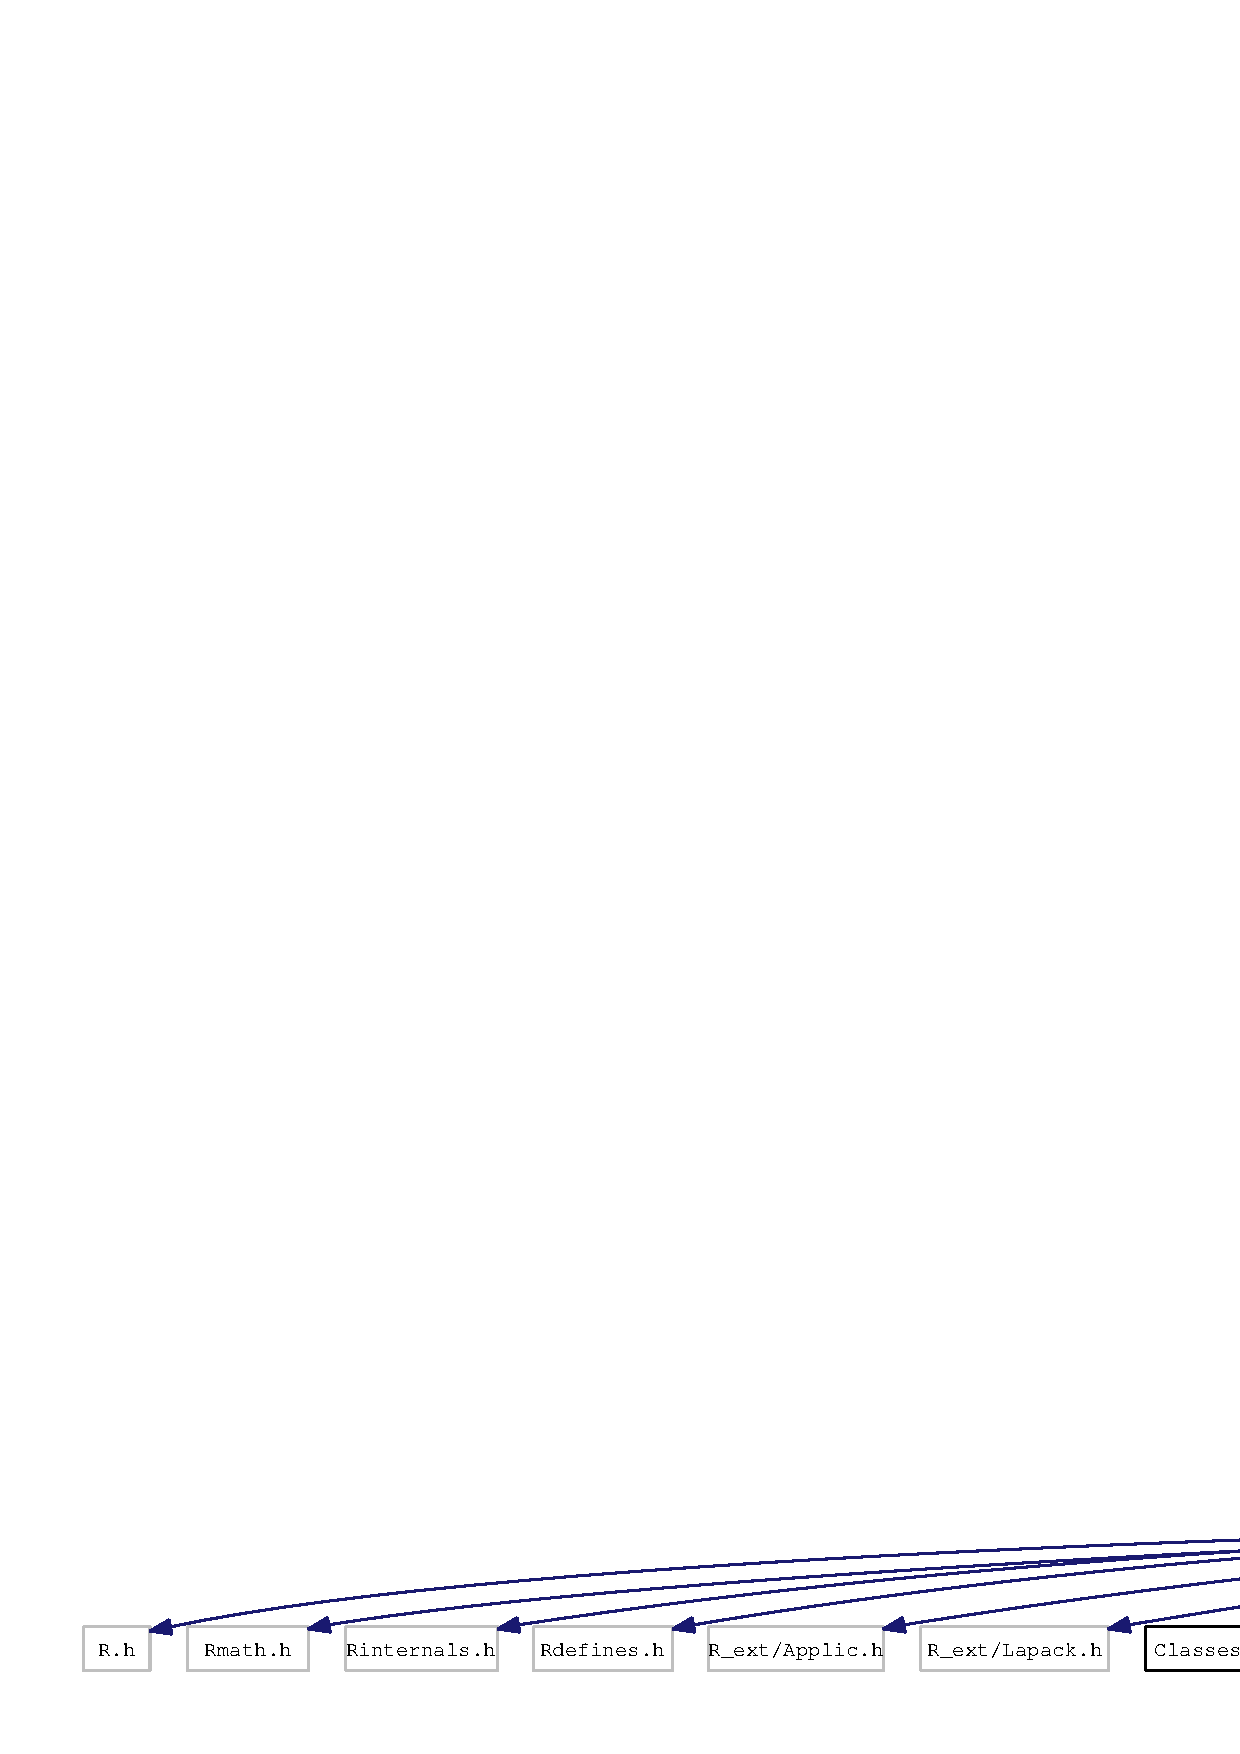
\includegraphics[width=420pt]{TestStatistic_8c__incl}
\end{center}
\end{figure}
\subsection*{Functions}
\begin{CompactItemize}
\item 
void \hyperlink{TestStatistic_8c_9ecf0700a00ad5fd64601bf718f20439}{C\_\-standardize} (const double $\ast$t, const double $\ast$mu, const double $\ast$Sigma, int pq, double tol, double $\ast$ans)
\item 
void \hyperlink{TestStatistic_8c_6939f019d2c7f42ae824776043a8c704}{C\_\-absstandardize} (const double $\ast$t, const double $\ast$mu, const double $\ast$Sigma, int pq, double tol, double $\ast$ans)
\item 
double \hyperlink{TestStatistic_8c_a3a1f48e4bb3aa19d1bac85a53358638}{C\_\-maxabsTestStatistic} (const double $\ast$t, const double $\ast$mu, const double $\ast$Sigma, int pq, double tol)
\item 
SEXP \hyperlink{TestStatistic_8c_499b26b98aaf073dc66135ecde8ad851}{R\_\-maxabsTestStatistic} (SEXP t, SEXP mu, SEXP Sigma, SEXP tol)
\item 
double \hyperlink{TestStatistic_8c_b45eb88ec3b2cc87e8610771cdcf53c4}{C\_\-quadformTestStatistic} (const double $\ast$t, const double $\ast$mu, const double $\ast$SigmaPlus, int pq)
\item 
SEXP \hyperlink{TestStatistic_8c_825d2b1db2c719f8d1c2e2ec3f79e1a4}{R\_\-quadformTestStatistic} (SEXP t, SEXP mu, SEXP SigmaPlus)
\end{CompactItemize}


\subsection{Detailed Description}
Test statistics for conditional inference

\begin{Desc}
\item[Author:]\begin{Desc}
\item[Author]\end{Desc}
\end{Desc}
\begin{Desc}
\item[Date:]\begin{Desc}
\item[Date]\end{Desc}
\end{Desc}


Definition in file \hyperlink{TestStatistic_8c-source}{TestStatistic.c}.

\subsection{Function Documentation}
\hypertarget{TestStatistic_8c_6939f019d2c7f42ae824776043a8c704}{
\index{TestStatistic.c@{TestStatistic.c}!C_absstandardize@{C\_\-absstandardize}}
\index{C_absstandardize@{C\_\-absstandardize}!TestStatistic.c@{TestStatistic.c}}
\subsubsection{\setlength{\rightskip}{0pt plus 5cm}void C\_\-absstandardize (const double $\ast$ {\em t}, const double $\ast$ {\em mu}, const double $\ast$ {\em Sigma}, int {\em pq}, double {\em tol}, double $\ast$ {\em ans})}}
\label{TestStatistic_8c_6939f019d2c7f42ae824776043a8c704}


Absolute values of standardized statistics \begin{Desc}
\item[Parameters:]
\begin{description}
\item[{\em t}]the vector of statistics \item[{\em mu}]expectations \item[{\em Sigma}]covariance matrix \item[{\em pq}]dimension of t \item[{\em tol}]tolerance for variances \item[{\em ans}]return value; a pointer to a REALSXP-vector of length pq \end{description}
\end{Desc}


Definition at line 49 of file TestStatistic.c.

References C\_\-abs(), and C\_\-standardize().

Referenced by C\_\-maxabsTestStatistic().

Here is the call graph for this function:\nopagebreak
\begin{figure}[H]
\begin{center}
\leavevmode
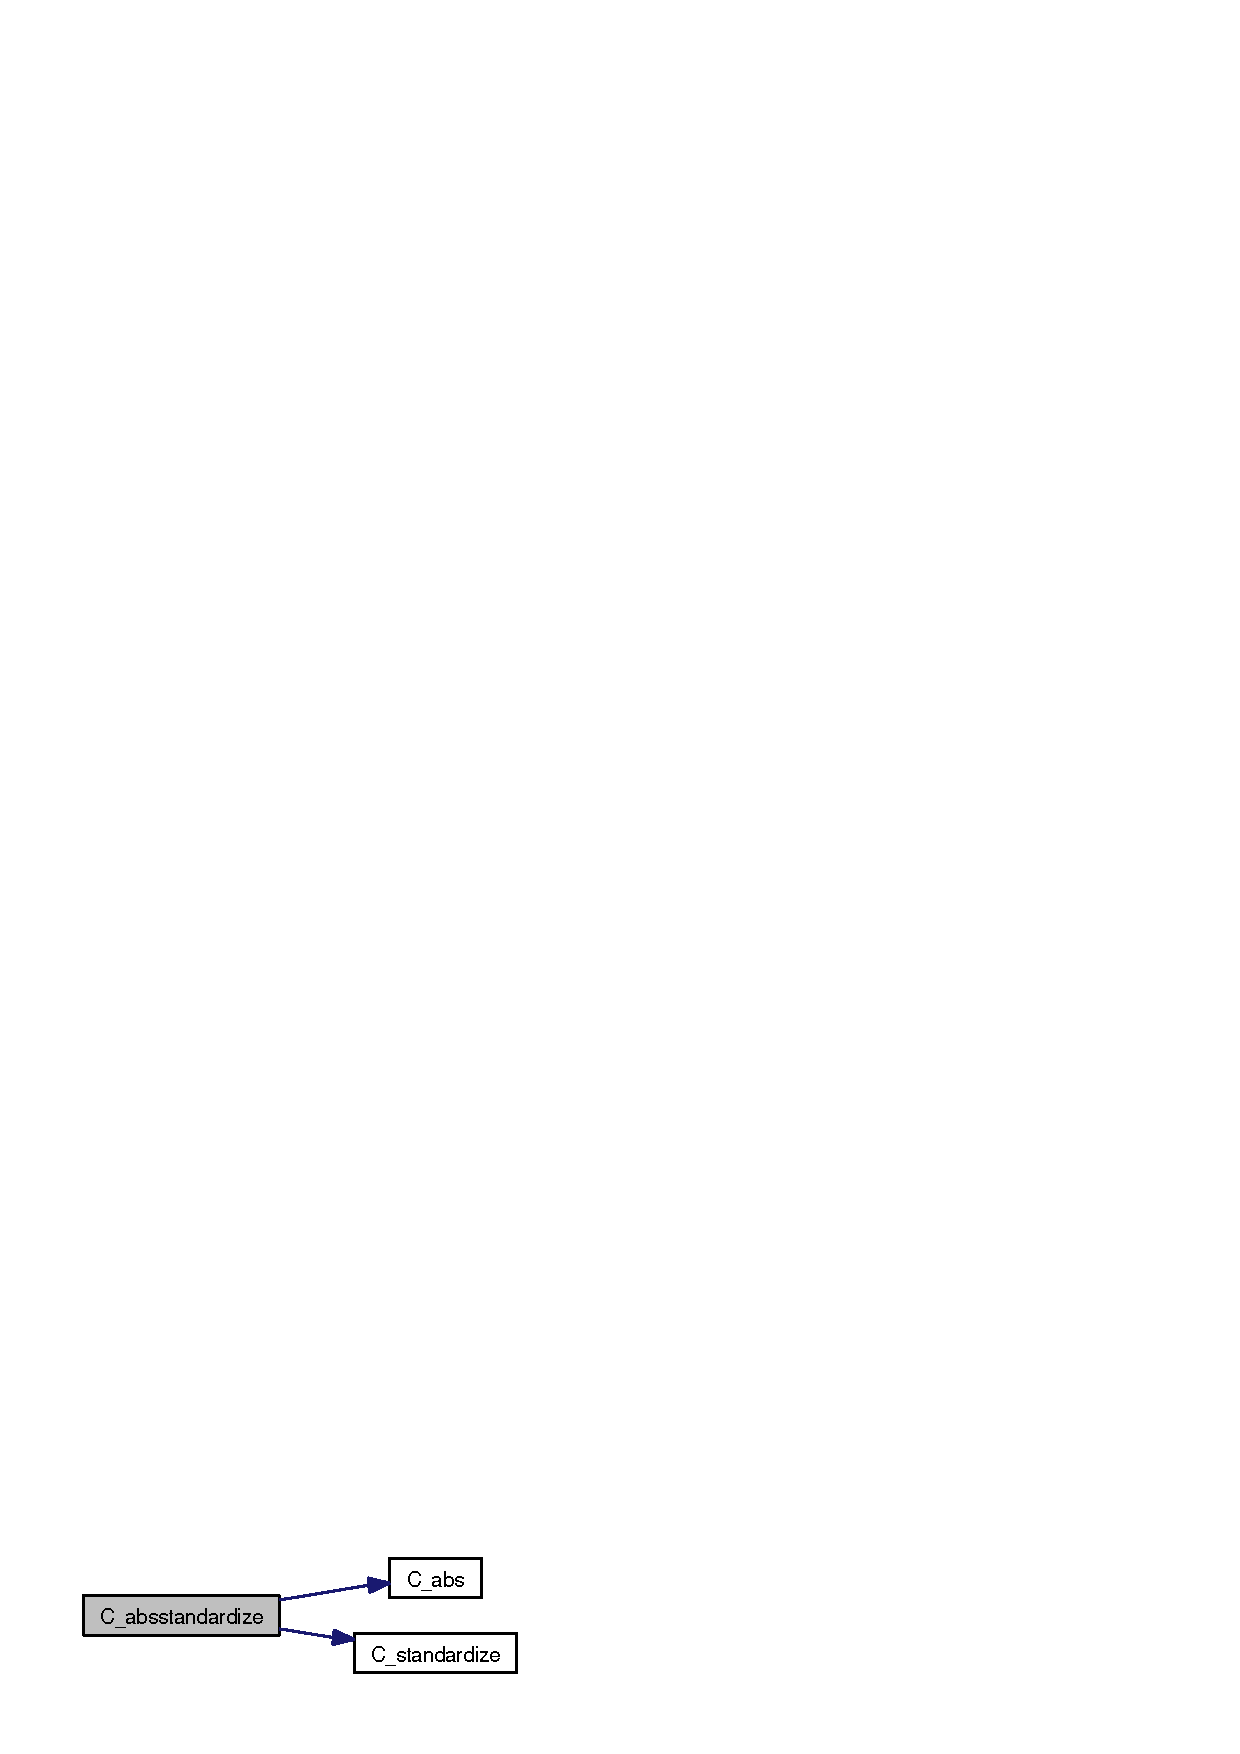
\includegraphics[width=134pt]{TestStatistic_8c_6939f019d2c7f42ae824776043a8c704_cgraph}
\end{center}
\end{figure}
\hypertarget{TestStatistic_8c_a3a1f48e4bb3aa19d1bac85a53358638}{
\index{TestStatistic.c@{TestStatistic.c}!C_maxabsTestStatistic@{C\_\-maxabsTestStatistic}}
\index{C_maxabsTestStatistic@{C\_\-maxabsTestStatistic}!TestStatistic.c@{TestStatistic.c}}
\subsubsection{\setlength{\rightskip}{0pt plus 5cm}double C\_\-maxabsTestStatistic (const double $\ast$ {\em t}, const double $\ast$ {\em mu}, const double $\ast$ {\em Sigma}, int {\em pq}, double {\em tol})}}
\label{TestStatistic_8c_a3a1f48e4bb3aa19d1bac85a53358638}


Maximum absolute values of standardized statistics \begin{Desc}
\item[Parameters:]
\begin{description}
\item[{\em t}]the vector of statistics \item[{\em mu}]expectations \item[{\em Sigma}]covariance matrix \item[{\em pq}]dimension of t \item[{\em tol}]tolerance for variances \end{description}
\end{Desc}


Definition at line 66 of file TestStatistic.c.

Referenced by C\_\-TestStatistic(), and R\_\-maxabsTestStatistic().\hypertarget{TestStatistic_8c_b45eb88ec3b2cc87e8610771cdcf53c4}{
\index{TestStatistic.c@{TestStatistic.c}!C_quadformTestStatistic@{C\_\-quadformTestStatistic}}
\index{C_quadformTestStatistic@{C\_\-quadformTestStatistic}!TestStatistic.c@{TestStatistic.c}}
\subsubsection{\setlength{\rightskip}{0pt plus 5cm}double C\_\-quadformTestStatistic (const double $\ast$ {\em t}, const double $\ast$ {\em mu}, const double $\ast$ {\em SigmaPlus}, int {\em pq})}}
\label{TestStatistic_8c_b45eb88ec3b2cc87e8610771cdcf53c4}


Quadratic form t(t - mu) SigmaPlus (t - mu) \par
 \begin{Desc}
\item[Parameters:]
\begin{description}
\item[{\em t}]the vector of statistics \item[{\em mu}]expectations \item[{\em SigmaPlus}]Moore-Penrose inverse \item[{\em pq}]dimension of t \end{description}
\end{Desc}


Definition at line 110 of file TestStatistic.c.

Referenced by C\_\-TestStatistic(), and R\_\-quadformTestStatistic().\hypertarget{TestStatistic_8c_9ecf0700a00ad5fd64601bf718f20439}{
\index{TestStatistic.c@{TestStatistic.c}!C_standardize@{C\_\-standardize}}
\index{C_standardize@{C\_\-standardize}!TestStatistic.c@{TestStatistic.c}}
\subsubsection{\setlength{\rightskip}{0pt plus 5cm}void C\_\-standardize (const double $\ast$ {\em t}, const double $\ast$ {\em mu}, const double $\ast$ {\em Sigma}, int {\em pq}, double {\em tol}, double $\ast$ {\em ans})}}
\label{TestStatistic_8c_9ecf0700a00ad5fd64601bf718f20439}


Standardizes a statistic t of length pq with mean mu and covariance Sigma for variances $>$ tol \par
 \begin{Desc}
\item[Parameters:]
\begin{description}
\item[{\em t}]the vector of statistics \item[{\em mu}]expectations \item[{\em Sigma}]covariance matrix \item[{\em pq}]dimension of t \item[{\em tol}]tolerance for variances \item[{\em ans}]return value; a pointer to a REALSXP-vector of length pq \end{description}
\end{Desc}


Definition at line 23 of file TestStatistic.c.

Referenced by C\_\-absstandardize(), C\_\-Node(), and R\_\-splitcategorical().\hypertarget{TestStatistic_8c_499b26b98aaf073dc66135ecde8ad851}{
\index{TestStatistic.c@{TestStatistic.c}!R_maxabsTestStatistic@{R\_\-maxabsTestStatistic}}
\index{R_maxabsTestStatistic@{R\_\-maxabsTestStatistic}!TestStatistic.c@{TestStatistic.c}}
\subsubsection{\setlength{\rightskip}{0pt plus 5cm}SEXP R\_\-maxabsTestStatistic (SEXP {\em t}, SEXP {\em mu}, SEXP {\em Sigma}, SEXP {\em tol})}}
\label{TestStatistic_8c_499b26b98aaf073dc66135ecde8ad851}


R-interface to C\_\-maxabsTestStatistic \begin{Desc}
\item[Parameters:]
\begin{description}
\item[{\em t}]the vector of statistics \item[{\em mu}]expectations \item[{\em Sigma}]covariance matrix \item[{\em tol}]tolerance for variances \end{description}
\end{Desc}


Definition at line 87 of file TestStatistic.c.

References C\_\-maxabsTestStatistic().

Here is the call graph for this function:\nopagebreak
\begin{figure}[H]
\begin{center}
\leavevmode
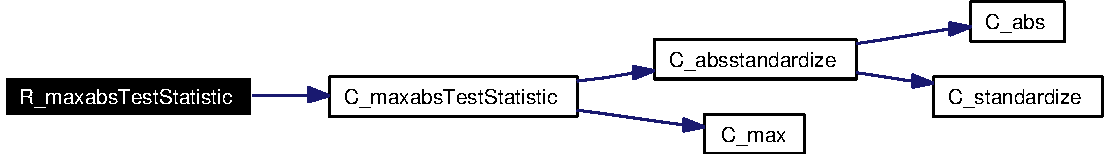
\includegraphics[width=165pt]{TestStatistic_8c_499b26b98aaf073dc66135ecde8ad851_cgraph}
\end{center}
\end{figure}
\hypertarget{TestStatistic_8c_825d2b1db2c719f8d1c2e2ec3f79e1a4}{
\index{TestStatistic.c@{TestStatistic.c}!R_quadformTestStatistic@{R\_\-quadformTestStatistic}}
\index{R_quadformTestStatistic@{R\_\-quadformTestStatistic}!TestStatistic.c@{TestStatistic.c}}
\subsubsection{\setlength{\rightskip}{0pt plus 5cm}SEXP R\_\-quadformTestStatistic (SEXP {\em t}, SEXP {\em mu}, SEXP {\em SigmaPlus})}}
\label{TestStatistic_8c_825d2b1db2c719f8d1c2e2ec3f79e1a4}


R-interface to C\_\-quadformTestStatistic \par
 \begin{Desc}
\item[Parameters:]
\begin{description}
\item[{\em t}]the vector of statistics \item[{\em mu}]expectations \item[{\em SigmaPlus}]Moore-Penrose inverse \end{description}
\end{Desc}


Definition at line 140 of file TestStatistic.c.

References C\_\-quadformTestStatistic().

Here is the call graph for this function:\nopagebreak
\begin{figure}[H]
\begin{center}
\leavevmode
\includegraphics[width=174pt]{TestStatistic_8c_825d2b1db2c719f8d1c2e2ec3f79e1a4_cgraph}
\end{center}
\end{figure}
